\section{Tracking}
\label{sec:tracking}
% !TeX spellcheck = en_US

Tracking is the most riveting part of the guide.
Haha.
No, not really.
It is probably the most mundane part of this whole thing, but twice as important as it is dry.
This insanely complex topic can be summed up with: \emph{do the damn tracking}.

And this it is, you are done.
You now have the broadest understanding about tracking and can get on with it in \tfn.
But perhaps you feel like reading on\ldots

\subsection{Main View: Tracker Sheet}
\label{subsec:main-tracker-sheet}

The sheet named \sheetname{Tracker} is the main data hub for the whole file.
Every piece of information in regards to tracking and budgeting is connected to a cell in this sheet.
As mentioned in \autoref{subsec:first-things-first}, the file is for 1 year, \ie 12 months.
You find the months spanning along the columns while the rows list income and expense classes.

\subsection{Categories}
\label{subsec:tracking-categories}

A good structure of categories of income and spending is the key to a good overlook and understanding of your finances.
As stated before, do what works best \emph{for you}!
If you want to, you can change up the way/pattern by which you name the tracking sheets.

I suggest to split up your spending into as many categories as possible.
For the day-to-day stuff I created the overarching class/group named \sterm{Daily}.
This class contains multiple categories, such as expenses in regards to groceries, bath \& household, food, clothing and miscellaneous items.
Hence I have the tracking sheets \sheetname{DailyGroceries} and \sheetname{DailyBathHousehold} attributed to it, as shown in \autoref{fig:tracking-categories}.

\begin{figure}[htp]
	\centering
	\includegraphics{Gfx/Introduction-Tracking-Categories.pdf}
	\caption[Tracking Categories]{These are some of the classes and their categories in Finances.ods.
	They are typical in certain fields of life, ordered by priority and frequency.
	You may create and name your own collection of classes and categories in any way you wish.%
	}
	\label{fig:tracking-categories}
\end{figure}

There are further elaborations to be given:
the classes and their categories are just an excerpt from my own version of \tfn, which is also somewhat incorporated into the file you downloaded.
I have a day-to-day life that the class \sterm{Daily} is for and I am sure its categories are self-explanatory.
The sheet \sheetname{MiscDaily} is a sheet that welcomes all stranger things that do not fit elsewhere.
And it is in fact the sheet that contains all \sterm{miscellaneous} things that do not fit in other classes/categories.
And at work, I need to buy food and drinks as well, so you will find that and other relevant categories in the \sterm{Work} class.

These categories are arguably quite granular and thus plentiful, which is how the structure developed over time, iterated with each edit.
I suppose one can say that I chose a strategy to mirror life in typical areas and split them up.\footnote{The \emph{very first} division of expense categories was inspired by the categories of a spreadsheet by \href{https://www.vertex42.com/}{Vertex42.com}, namely an old version of the Personal Budget Template.}

As stated a few times already, the content in the file is editable.
Hence the fields and their categories shown in \autoref{fig:tracking-categories} are to be understood as examples.
If you wish to do so, you can change it up to make it fit your needs.

Perhaps create a truly broad category structure, \ie make a class named something like \sterm{Living Expenses} with categories such as Rent, Electricity, Water, Groceries, etc..
Another class could \sterm{Recreational} for all kinds of expenses which occur because of activities and spending in/for leisure time.\footnote{This system is used by the reddit user \href{https://www.reddit.com/r/personalfinance/comments/aayvms/oc_i_tracked_every_dollar_i_spent_over_the_last_8/}{WhiskeySauer}.}

Or, one could maybe start by putting all monthly bills into the same field \sterm{Bills}, \ie you would end up with sheets like \sheetname{CableTV}, \sheetname{Internet} and \sheetname{InsuranceCar}, etc., regardless of the underlying reason how that bill came to be.
And expenses for different kinds of clothing could be grouped up into a class \emph{Clothing}, and thus have sheet names like \sheetname{WorkClothes}, \sheetname{ChildrenClothes} and so forth.
And the same could be done for different kinds of food, as you obviously need to eat, whether you are at home, work or at school.

Granted, some possibilities can be a bit silly and might prove to be counterproductive to going about this pragmatically or some really approach.
Whatever.
I am sure you already have a good idea of what you want and that is great, because it ultimately is up to you.
For the technicalities of adding, removing or editing categories, go to \autoref{subsec:editing-tracking-categories}.

\subsection{What to Track?}
\label{subsec:what-to-track}

You may find yourself wondering on what exactly it is you should and/or could track with \tfn.
Well, as stated before, I originally thought to track my cash.
And this is what the file primarily does.
But besides that, you can of course edit the file to include other kinds of wealth assets as well.

\subsection{How To Enter Tracking Data}
\label{subsec:enter-tracking-data}

There are \sterm{tracking sheets} for entering data on your expenses and income.
These sheets simply contain data which is to be put into 3 columns: date, description and amount.
Their layout and basic usage is shown in \fullref{fig:expenses-data-entry-in-sheet-moblity-car-gas}.

\begin{figure}[htp]
	\centering
	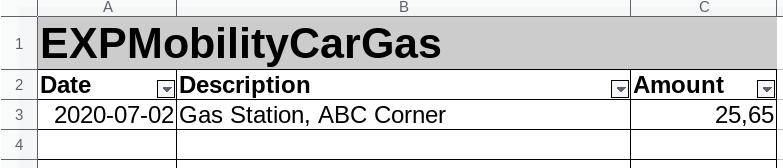
\includegraphics[width=0.8\linewidth]{Gfx/EXP-in-one-sheet-moblity-car-gas}
	\caption{Tracking Sheet for One Special Expense Category}
	\label{fig:expenses-data-entry-in-sheet-moblity-car-gas}
\end{figure}

\subsubsection{Tracking Column: Date}
\label{subsec:tracking-column-date}

Date: Enter the date for the day the expense occurred.
You can do this in two ways:
\begin{enumerate}
	\item Put the date for the day you made the expense or ordered it (online).
	\item Or--in case you pay with electronic cash, \eg via card--you might put the date the expense's value is actually transferred from your account.
	This might happen in the case of weekends, bank holidays or due to other kinds of service delays for money transfers.
\end{enumerate}

I \emph{strongly} suggest you use the first kind of date, as the date represents the better point in time, \ie the one you planned for.\footnote{This topic will be referenced and elaborated on in \autoref{subsubsec:different-dates-in-real-life}, \autopageref{subsubsec:different-dates-in-real-life}.}
Regardless, you should stay consistent in the method you choose.
The date does get checked for month and day, but not for the year, as I thought to use \tfn for 1 calendar year and have done so ever since.
So be careful that you enter the correct date as that timestamp is used to assign the amount to the right month.
And:
\begin{specialnote}
	Do not lie about the date.
\end{specialnote}

For writing the date into a cell, use the format \codestuff{YYYY-MM-DD} based on the international standard \href{https://en.wikipedia.org/wiki/ISO_8601}{ISO 8601}.
An example for July 4th, 2020: \codestuff{2020-07-04}.
It will help with the visual effect on quickly grasping which month and/or month you are looking at.
It is also incredibly easy to write if you have a numpad on your keyboard.
Also, who does not like a well-sorted list which looks equally properly formatted?? :)

But if you want to change the date format, simply edit the corresponding cell style template to produce the output you wish.
Note: as intended by the mechanism for style templates, this change would affect \emph{all} cells in the entire file which are formatted with this cell style-template.
And if you change the formatting, all formulas which work with dates have to be proof-checked (and possibly updated) as well.

\subsubsection{Tracking Column: Description}
\label{subsec:tracking-column-description}

Put down anything sensible that is coherent enough to make you remember, \eg ``Supermarket, Smith Street'', ``Gift coupon for John's 45th birthday, Macy's, Smith Street'' and so forth.

\subsubsection{Tracking Column: Amount}
\label{subsec:tracking-column-amount}

Put the amount that is to be attributed to this tracking sheet (and subsequently its category).
In relation to the bits mentioned in \autoref{subsec:tracking-column-description}, these could go into \sheetname{DailyGroceries} and \sheetname{DailyGifts}.
How and why these sheets have these names, all that was explained in \autoref{subsec:tracking-categories}, \autopageref{subsec:tracking-categories}.

If you want to change the format of the figures and have the symbol for your currency displayed, simply edit the corresponding cell style template to produce the output you wish.
Note: as intended by the mechanism for style templates, this change would affect \emph{all} cells in the entire file which are formatted with this cell style-template.

\subsection{Receipts and Documentation}
\label{subsec:tracking-receipts}

Collect your receipts, bills, notes and whatever you have that documents the amounts you paid.\footnote{Maybe put them on/in some kind of holder/retainer thing.}
As soon as you worked through a receipt and split up its content into your spending categories, mark it or throw it away instantly, unless you might need it again.
If you think that you might need the receipt in the future, \eg for tax purposes or for perhaps returning the item, put them in another kind of documentation envelope/folder.\footnote{Maybe collect them in a shoebox, an envelope or in a plastic pocket.}

Also, go through your monthly bank statements line by line and check them off.
This most likely leads to delayed entries in the tracking sheets but it ensures factually correct tracking data.

\subsection{Workload}
\label{subsec:tracking-workload}

In a way, entering all the data could be interpreted as work.
In my experience, I am content with updating \tfn at least every second week.
Of course it would still work fine to update it every second, third or fourth week as well.

\subsection{Splitting Receipts}
\label{subsec:splitting-receipts}

If you shopped at a store where you bought multiple kinds of various items, you take the amounts spent in different categories and write them into the respective tracking sheets for these categories and name the entries accordingly.

\subsection{Examples for Entering Tracking Data}
\label{subsec:examples-for-entering-tracking-data}

Say you went to Aldi and you spent a total amount of 30.65\,€.
You bought groceries and supplies for the household.
This could be an entry in the sheet for groceries then:
\begin{center}\sffamily
	\begin{tabular}{|l|l|r|}
		\multicolumn{3}{l}{Groceries}\\
		\hline
		\textbf{Date} & \textbf{Description} & \textbf{Amount}\rmfamily\\
		\hline
		2018-06-01 & Aldi, ABC Street tot. 30.65 & 19.13\\
		\hline
	\end{tabular}
\end{center}

The remainder of \( 30.65 - 19.13 = 11.52\) is to be billed to another category, in this case Household \& Bath Supplies.
So again you go the relevant sheet and enter the data accordingly:
\begin{center}\sffamily
	\begin{tabular}{|l|l|r|}
		\multicolumn{3}{l}{Household \& Bath Supplies}\\			
		\hline
		\textbf{Date} & \textbf{Description} & \textbf{Amount}\\
		\hline
		2018-06-01 & Aldi, ABC Street tot. 30.65 & 11.52\\
		\hline
	\end{tabular}
\end{center}

\subsection{An Alternative Way of Grouping Tracking Data}
\label{subsec:alternative-way-of-grouping-tracking-data}

There is at least one other way of enter tracking data, which is to gather all the expense/income data in one sheet only.
To showcase an example that alternative way of grouping tracking data, take a look at \fullref{fig:expenses-data-entry-in-one-sheet-only}.
I originally considered using this system but it proved to be too burdensome in the long run.
\begin{figure}[htp]
	\centering
	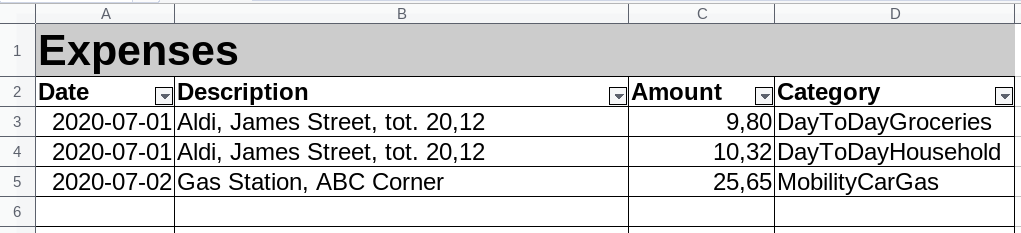
\includegraphics[width=0.8\linewidth]{Gfx/EXP-all-in-one-sheet}
	\caption{Tracking Sheet for All Expenses}
	\label{fig:expenses-data-entry-in-one-sheet-only}
\end{figure}

I am not using that system for the following reasons:
\begin{enumerate}
	\item If you want to take a look at spending data, it is beneficial to need as little time and effort as possible to get to it.
	Doing that in the alternative way, you would have to scroll and filter more, relatively speaking.
	\item If you intend to change something about my expenses categories, you need to rename the category in \sheetname{Tracker} and the actual sheetname.
	In case of grouping all expenses, you would have to change the category name first, then look for all entries in the tracking sheet and refill the category entry.
	To be fair, also renaming the budget categories for budgeted items is a given in both cases.
	\item In case of an accident with deleting or overwriting data, only the tracking data in one sheet could be damaged.
\end{enumerate}
All systems certainly have their advantages and drawback.
In any case, that should not stop you from entering and structuring the data in some other way.
If you like to, please be aware that \tfn and this document might not be the best fit for your needs then, if at all.

If you want to use an alternative way, there are other possibilities available.
As far as I can tell, grouping of all expenses/income in one sheet is used/provided by the reddit user \href{https://www.reddit.com/user/getToTheChopin/}{getToTheChopin}.
Their content is available on \url{https://themeasureofaplan.com}.

\subsection{Different Values in Finances.ods vs. Real-World Data}
\label{subsec:different-values-finances.ods-vs-real-world}

One basic understanding for working with \tfn is that there is going to be a difference between the amounts which are displayed in \tfn on the one hand, and all the numbers from the accounts that you decided you track (most definitely the account you use for your salary/wage being one of them).
I regard this as inevitable.
However thorough your notes and collection of receipts are, keep in mind that it is totally and entirely normal thing to misremember or forget.

You need to decide if a difference in the single digit-range (although I sincerely doubt this is possible) is acceptable or if you are still ok with low three digits, or perhaps even more.
Before you go ahead and calculate the different, take a look at which items make up the difference:
\begin{itemize}
	\item balance in the accounts your are tracking
	\item the amount of cash in your wallet
	\item the amount of cash that each person with access to the tracked accounts has
\end{itemize}